% ============================================================================
%  Sinhala-ABD content for the SAID data paper.
%
%  Drop-in replacements, marked below. Nothing here reports detector results:
%  this is dataset-description material only.
%
%  CONTENTS
%    [1] Table 1 (tab:overview) -- replace wholesale
%    [2] "Sinhala-ABD" paragraph in Construction -- replaces the \ph{...} stub
%    [3] Table: ABD composition -- new
%    [4] Figures 1 and 2 for ABD -- new
%    [5] Validation subsection for ABD -- append to Section 4
%    [6] Limitations sentences -- merge into Section 6
%    [7] Worked example -- replaces the \ph{...} in Appendix C
%
%  Every number is measured from the released corpus.
% ============================================================================


% ---------------------------------------------------------------------------
% [1] REPLACES the existing tab:overview
% ---------------------------------------------------------------------------
\begin{table}[!b]
\centering\small
\caption{Overview and scale of the two Sinhala datasets.}
\label{tab:overview}
\begin{tabular}{@{}p{0.12\linewidth}p{0.43\linewidth}p{0.38\linewidth}@{}}
\toprule
 & \textbf{Sinhala-HAT} & \textbf{Sinhala-ABD} \\
\midrule
Task & Human vs.\ AI classification & Sentence labels and boundaries \\
Domains & News, Wikipedia, social media & Wikipedia \\
Scale & 4{,}500 human--AI pairs; 9{,}000 documents & 4{,}244 mixed documents; 39{,}358 labelled sentences \\
 & 1{,}500 pairs per domain & 2{,}630 source articles \\
 & 500 pairs per generator per domain & 14{,}318 machine sentences (36.4\%) \\
\bottomrule
\end{tabular}
\end{table}


% ---------------------------------------------------------------------------
% [2] REPLACES the "\paragraph{Sinhala-ABD.}" paragraph, including its \ph{}
% ---------------------------------------------------------------------------
\paragraph{Sinhala-ABD.}
Mixed documents are built from contiguous Wikipedia passages of six to twelve
sentences, cut from articles that survive a page-type and prose filter
(Appendix~\ref{app:abd-cleaning}). Every sentence carries a human or machine
label, and boundaries are derived from the label sequence rather than stored
separately, so a boundary is by definition an index where the label changes.
Figure~\ref{fig:abd-constructions} shows the three document types.
In \emph{continuation}, a split point is sampled uniformly between 20\% and 80\%
of the passage; the true remainder is discarded and the model writes a
replacement conditioned on the prefix. In \emph{single-span replacement}, one
internal span of one to three sentences is rewritten, with the model shown the
left and right context but instructed to rewrite only the marked span. In
\emph{multi-span replacement}, two or three non-adjacent spans of one to two
sentences are rewritten, each generated \emph{independently from the original
human passage} rather than sequentially, so the model cannot impose a single
consistent machine register across the document; all spans in a document come
from one generator. Spans may not include the first or last sentence, and at
least one human sentence separates consecutive spans, so replacement never
degenerates into a prefix or suffix change. The 20--80\% sampling and the
first/last-sentence rule exist to stop position alone from identifying
boundaries; the resulting distribution is shown in
Figure~\ref{fig:abd-positions}. Documents are never padded into a longer type:
a passage too short for a construction is simply ineligible for it.
Table~\ref{tab:abd-composition} gives the composition. Sinhala-ABD is
constructed independently of Sinhala-HAT, although human source texts may
overlap between the two datasets.


% ---------------------------------------------------------------------------
% [3] NEW -- place after the Sinhala-ABD paragraph
% ---------------------------------------------------------------------------
\begin{table}[tb]
\centering\small
\caption{Sinhala-ABD composition. Machine share is the mean proportion of
machine sentences per document. Gemini~2.5~Pro is generated for a disjoint
subset of source articles, supporting leave-one-generator-out evaluation.}
\label{tab:abd-composition}
\begin{tabular}{@{}lrrrr@{}}
\toprule
\textbf{Construction} & \textbf{Docs} & \textbf{Sentences} & \textbf{Boundaries/doc} & \textbf{Machine share} \\
\midrule
Continuation           & 1{,}675 & 15{,}122 & 1.00 & 49.4\% \\
Single-span replacement & 1{,}367 & 12{,}398 & 2.00 & 24.5\% \\
Multi-span replacement  & 1{,}202 & 11{,}838 & 4.97 & 33.0\% \\
\midrule
\textbf{Total}          & \textbf{4{,}244} & \textbf{39{,}358} & 2.45 & 36.4\% \\
\midrule
\multicolumn{5}{@{}l}{\textit{By generator}} \\
GPT-4o                 & 1{,}898 & & & \\
DeepSeek~V3            & 1{,}761 & & & \\
Gemini~2.5~Pro         & 585 & & & \\
\bottomrule
\end{tabular}
\end{table}


% ---------------------------------------------------------------------------
% [4] NEW -- figures
% ---------------------------------------------------------------------------
\begin{figure}[tb]
\centering
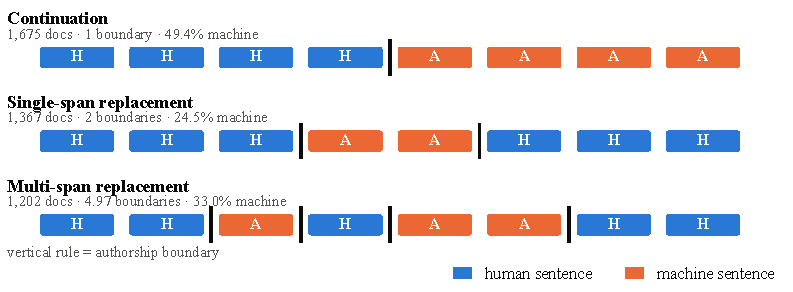
\includegraphics[width=\linewidth]{figures/abd_fig1_constructions.pdf}
\caption{The three Sinhala-ABD construction types, with corpus statistics.
Replacement keeps the surrounding text genuinely human-written and constrains
the generated passage to the content it replaces. Spans never include the first
or last sentence, and consecutive spans are separated by at least one human
sentence.}
\label{fig:abd-constructions}
\end{figure}

\begin{figure}[tb]
\centering
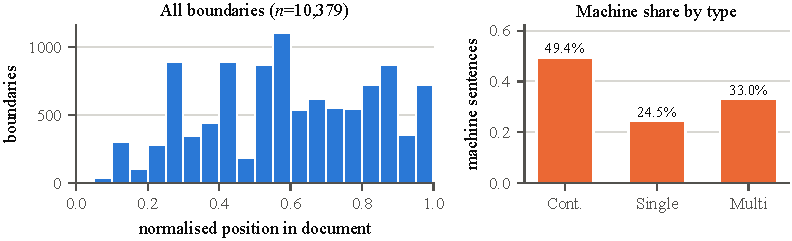
\includegraphics[width=\linewidth]{figures/abd_fig2_positions.pdf}
\caption{Left: normalised positions of all 10{,}379 authorship boundaries. The
distribution is spread rather than concentrated, so position alone does not
identify a boundary, though the construction rules leave it non-uniform. Right:
mean machine-sentence share by construction type.}
\label{fig:abd-positions}
\end{figure}


% ---------------------------------------------------------------------------
% [5] APPEND to Section 4 (Validation), after the two existing paragraphs
% ---------------------------------------------------------------------------
\paragraph{Automatic validation of Sinhala-ABD.}
Because a mixed document's labels are only correct if the generated span is
actually usable in place of the text it replaced, every generation passes seven
automatic checks before it enters the corpus: exact sentence count; word count
within $\pm$25\% of the replaced span; no preamble; no Markdown; predominantly
Sinhala script; not a near-copy of the original span under normalised
comparison; and preservation of numeric tokens, so a date or quantity cannot
silently mutate. A failing generation is retried up to three times and then
discarded, and outputs are never edited by hand, so the corpus contains only
text the generators actually produced. Across 5{,}109 rejected generations, which record 5{,}951 individual check
failures since one generation may fail several checks at once, 53.7\% of
failures were length violations, 23.9\% sentence-count violations, 16.3\%
number mutations, 3.5\% script violations, 2.3\% near-copies, and 0.3\%
formatting. The length tolerance
was deliberately not relaxed: all three generators under-write Sinhala relative
to the human span, and admitting shorter machine spans would let sentence length
substitute for authorship as a detection signal. 76.8\% of accepted documents
passed on the first attempt, 15.2\% after one retry, and 8.0\% after two or
more.

\paragraph{Generator screening.}
Quality control is applied at the generator level rather than per example. A
fourth candidate generator, Mistral~Nemo, was piloted and rejected: it produced
malformed Sinhala word forms, repetition loops, and outputs in which the prompt
instructions themselves appeared as content. Critically, the small number of its
outputs that \emph{passed} the automatic checks showed the same defects, having
satisfied only the sentence and word counts. This is a limitation of automatic
validation worth stating plainly: the script check measures the proportion of
characters in the Sinhala Unicode block, so text composed of Sinhala characters
that is not Sinhala \emph{language} passes it. Format checks are not fluency
checks, and any generator added later must be read by a native speaker before
it is trusted. \ph{ABD: add native-speaker fluency results once the
Section~\ref{sec:validation} study covers ABD spans as well as HAT documents.}


% ---------------------------------------------------------------------------
% [6] MERGE into Section 6 (Limitations)
% ---------------------------------------------------------------------------
% Add these sentences to the Limitations section:
%
% Sinhala-ABD source articles are drawn from a current Wikipedia snapshot with
% no revision-date cutoff, because the distribution we use carries no revision
% timestamp. Unlike Sinhala-HAT, whose Wikipedia portion is taken as it stood
% before 1 January 2015, the human sentences in Sinhala-ABD therefore cannot be
% guaranteed to predate widespread LLM availability.
%
% Machine-sentence share differs by construction type (49.4\%, 24.5\%, 33.0\%),
% so results pooled across types are weighted by that imbalance and should be
% reported per type.
%
% Sinhala-ABD contains 585 Gemini~2.5~Pro documents against 1{,}898 and 1{,}761
% for the other two generators, so held-out-generator evaluation using Gemini
% rests on a smaller sample than the seen-generator comparison.


% ---------------------------------------------------------------------------
% [7] REPLACES the \ph{} in Appendix C (Worked example) -- ABD half only
% ---------------------------------------------------------------------------
\subsection*{A Sinhala-ABD mixed document}

Multi-span replacement, generated by DeepSeek~V3 from the article
\si{උගන්ඩාවේ භූගෝලය} (\emph{Geography of Uganda}). Labels are
$[0,0,1,0,1,0,1,0]$; H marks a human sentence and A a machine sentence. Three
single-sentence spans were each rewritten independently from the original
passage.

\begin{table}[h]
\centering\small
\begin{tabular}{@{}cl p{0.80\linewidth}@{}}
\toprule
\# & & Sentence \\
\midrule
0 & H & \si{එහි භූගෝලය ගිනිකඳු කඳු, කඳු සහ විල් වලින් සමන්විත ඉතා විවිධාකාර වේ.} \\[2pt]
1 & H & \si{රට සාමාන්‍යයෙන් මුහුදු මට්ටමේ සිට මීටර් 900 ක උසකින් පිහිටා ඇත.} \\[2pt]
2 & \textbf{A} & \si{උගන්ඩාවේ නැගෙනහිර හා බටහිර දෙපසම කඳුකරයන් පිහිටා ඇත.} \\[2pt]
3 & H & \si{රුවෙන්සෝරි කඳුවැටිය උගන්ඩාවේ උසම කඳු මුදුන අඩංගු වන අතර එය ඇලෙක්සැන්ඩ්‍රා ලෙස නම් කර ඇති අතර එහි විශාලත්වය මීටර් 5,094 කි.} \\[2pt]
4 & \textbf{A} & \si{රටේ දකුණු කොටසෙහි විශාල ප්‍රදේශයක් ලෝකයේ විශාලතම විල් ලෙස සැලකෙන වික්ටෝරියා විලේ බලපෑමට යටත්ව ඇති අතර එහි බොහෝ දූපත් දක්නට ලැබේ.} \\[2pt]
5 & H & \si{කම්පාලා අගනුවර සහ එන්ටෙබේ අගනුවර ඇතුළුව මෙම වැව ආසන්නයේ වඩාත් වැදගත් නගර දකුණේ පිහිටා ඇත.} \\[2pt]
6 & \textbf{A} & \si{රටේ මධ්‍යයේ පිහිටි කියෝගා විල පුළුල් වගුරු බිම් වලින් යුක්ත වේ.} \\[2pt]
7 & H & \si{ගොඩබිම් සහිත වුවද උගන්ඩාවේ විශාල විල් රාශියක් ඇත.} \\
\bottomrule
\end{tabular}
\end{table}

\noindent The machine sentences preserve the factual content of the spans they
replaced and match the surrounding encyclopedic register, so the boundaries are
not marked by any surface cue. Alternating single-sentence spans are the densest
configuration the corpus contains.


% ---------------------------------------------------------------------------
% [8] NEW APPENDIX -- Sinhala-ABD source filtering
% ---------------------------------------------------------------------------
\section{Sinhala-ABD source filtering}
\label{app:abd-cleaning}

Sinhala-ABD sources are drawn from the same \texttt{wikipedia-monthly} Sinhala
subset as Sinhala-HAT (26{,}470 articles). Cleaning operates on the raw wikitext
rather than the distribution's pre-extracted plain-text field, which retains
category lines, unexpanded template calls, and magic words, and which flattens
list markup into text that a sentence splitter cannot distinguish from prose.

Pages are removed if they are the main page, carry a non-article namespace
prefix, are redirects, are disambiguation pages (\si{බහුරුත්හරණය}), are marked
as stubs (\si{දියුණු කරන්න}), or are list pages identified by title or by
structure. Remaining pages must then pass a prose gate of at least 120 words and
at least eight sentences, and must be predominantly Sinhala script. Of 26{,}470
articles, 9{,}390 (35.5\%) survive; the prose gate accounts for most of the
loss, reflecting the size distribution of Sinhala Wikipedia, whose median
article is roughly 2{,}000 characters. Markup is then stripped in a fixed
order --- comments, references, tables, templates, file and category links,
interwiki links, then link and emphasis syntax --- and paragraphs are reflowed
according to MediaWiki semantics, in which a single newline inside a paragraph
is a soft wrap rather than a break. The 9{,}390 surviving articles yield 7{,}944
windows, of which 2{,}630 are used.

Sentence segmentation is deterministic and shared by every stage of the
pipeline, so sentence indices and labels cannot drift apart. It splits on
\texttt{.}, \texttt{?}, \texttt{!} and the kunddaliya (\si{෴}), with guards for
decimals and for abbreviations including \si{ආචාර්ය.} and \si{පෙ.ව.} The guard
for initials is restricted to ASCII letters: \si{ය} is a common Sinhala
sentence-final particle, and an unrestricted rule silently merges sentences
across the corpus.
